\chapter{Language Models}



\section{LSTM}

LSTM is used for question analyzing tasks. It can reserve the state of a sequence.

\begin{figure}[h!]
	\centering
	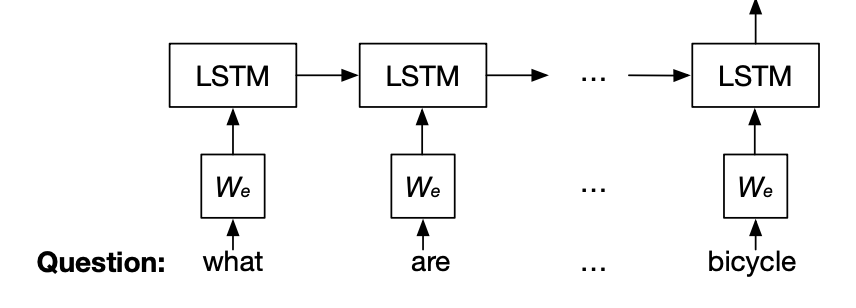
\includegraphics{img/lstm-example}
	\caption{LSTM based question model \textit{what are sitting in the basket on a bicycle.} \cite{SAN}}
	\label{fig:lstm}
\end{figure}

Given the question 
\[ q =[q_1, ..., q_T] \]
where $ q_t $ is the one hot vector representation of word at position $ t $.
We embedded the words to a vector space through an embedding matrix and get the input vector $ x_t $,
\[ x_t = W_e q_t, t\in \{1,2,...,T\}\]
Then for every time step, we feed the embedding vector of words in the question to LSTM, then output a hidden state $ h_t $,
\[h_t = LSTM(x_t), t\in \{1,2,...,T\} \]
The LSTM update process uses the gate mechanism. An input gate $ i_t $ controls how much the current input $ x_t $ updates the memory cell.
\[ i_t = \sigma (W_{xi} x_t + W_{hi} h_{t-1} + b_i  ) \]
The forget gate $ f_t $ controls how much information from past state $ c_{t-1} $ is preserved.
\[f_t = \sigma (W_{xf} x_t  + W_{hf}h_{t-1} + b_f) \]
The output gate $ o_t $ controls how much information of the memory is fed to the output as hidden state
\[ o_t = \sigma ( W_{xo} x_t + W_{ho} h_{t-1} + b_o ) \]
The memory cell $ c_t $ reserves the state of a sequence
\[ c_t = f_tc_{t-1}  + i_t\tanh (W_{xc}x_t + W_{hc} h_{t-1} + b_c)  \]
The output hidden state $ h_t $ is updated as 
\[h_t = o_t\tanh(c_t)\]
The final hidden layer is taken as the representation vector for the question, i.e.
\[v_Q = h_T\]

\section{CNN}

\begin{figure}[h!]
	\centering
	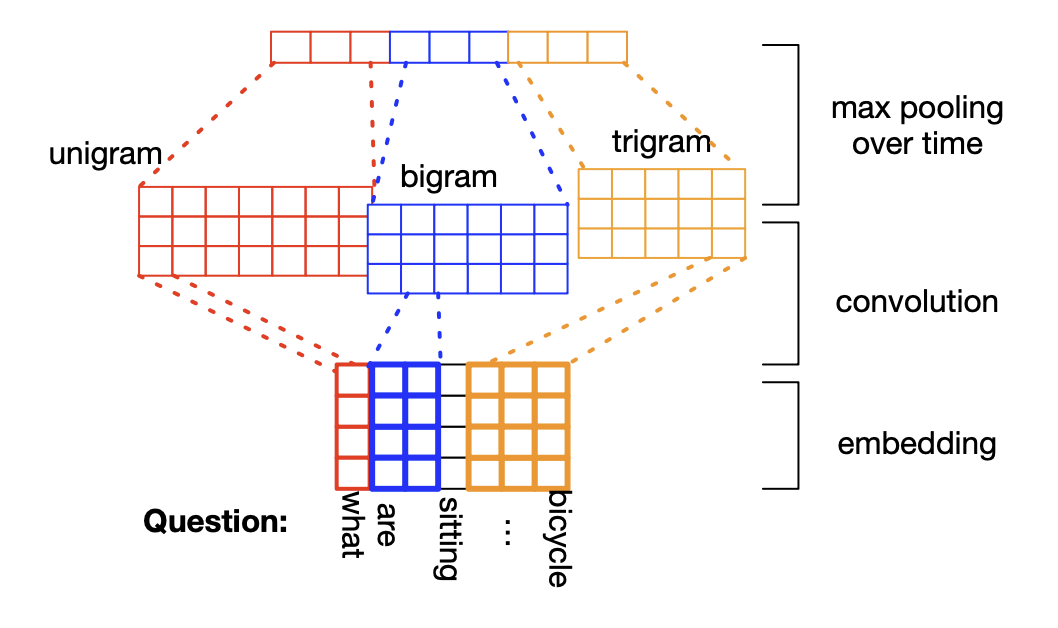
\includegraphics[width=\linewidth]{img/cnn-example}
	\caption{CNN based question model \textit{what are sitting in the basket on a bicycle.} \cite{SAN}}
	\label{fig:cnn-la}
\end{figure}


Similar to LSTM based model, CNN model embeds words to \textbf{word vectors}
\[x_t = W_e q_t \]
Then it concatenates the word vectors to \textbf{question vectors}
\[x_{1:T} = [x_1, x_2, ..., x_T]\]
Let  $ c $ denotes the size of convolution filters, $ t $ denotes the t-th convolution output, $ W_c $ is the convolution weight, $ b_c $ is the bias. The convolution output is given by
\[ h_{c, t} = \tanh(W_cx_{t:t+c-1}  + b_c )\]
The \textbf{feature map} with convolution filter size $ c $ is given by
\[h_c = [h_{c,1}, h_{c,2},..., h_{c, T-c+1}]\]
Then we apply max-pooling over the feature maps of the convolution size $ c $ and denote it as 
\[ \tilde{h}_c = \max_t[h_{c,1}, h_{c,2}, ..., h_{c, T-c+1}] \] 
For convolution feature maps of different sizes $ c $, we concatenate them to form the feature representation vector of the whole question sentence
\[h = [\tilde{h}_1, \tilde{h}_2, \tilde{h}_3]\]
Hence the CNN based question vector is
\[v_Q  = h\]


\section{Stacked Attention Networks (SAN)}
Let $ v_I\in \mathbb{R}^{d \times m} $ denotes the image feature matrix, $ m $ is the number of image regions. $ v_Q \in \mathbb{R}^d $ is a $ d $ dimensional vector. denotes the question feature vector. Let $ W_{I,A}, W_{Q,A} \in \mathbb{R}^{k\times d}$, $ \oplus $ denotes the addition of a matrix and a vector, which is performed by adding each column of the matrix by the vector. Then the two vectors first go through a single layer neural network
\[h_A = \tanh (W_{I,A}v_I \oplus (W_{Q,A}v_Q+b_A))\]
Let $ W_P \in \mathbb{R}^{1\times k} $, then a softmax function is used to generate the attention distribution $ p_I \in \mathbb{R}^m $ over the regions of the image, which corresponds to the attention probability of each image region given $ v_Q $.
\[p_I = \mbox{softmax}(W_Ph_A + b_P)\]
Based on the attention distribution we calculate the weighted sum of the image vectors $ \tilde{v}_i $. 
\[\tilde{v}_I  = \sum_i p_i v_i \]
Then $ \tilde{v}_i $ is combined with the question vector $ v_Q $ to form a refined \textbf{query vector} $ u $.
\[u = \tilde v_I + v_Q \]
The $ k $-th attention layer is calculated as 
\begin{equation}
\begin{split}
	h_A^k &= \tanh(W_{I, A}^k v_I \oplus (W^k_{Q,A}u^{k-1} + b^k_A))\\
	p^k_I  &= \mbox{softmax}(W^k_P h^k_A + b^k_P)
\end{split}
\end{equation}
where $ u^0 $ is initialized to be $ v_Q $. The aggregated image feature vector is added to the previous query vector to form a new query vector:
\begin{equation}
	\begin{split}
		\tilde{v}^k_I &= \sum_i p_i^k v_i\\
  		u^k &= \tilde{v}^k_I + u^{k-1}
	\end{split}
\end{equation}
It will be repeat for $ K $ times and then use the final $ u^K $ to infer the answer:
\[ p_{ans} = \mbox{softmax}(W_u u^K + b_u)\]

\section{Convolutional bottleneck attention module (CBAM)}
The CBAM\cite{CBAM} module is designed to learn what and where to emphasize or suppress and refines intermediate features effectively.
\begin{figure}[h!]
	\centering
	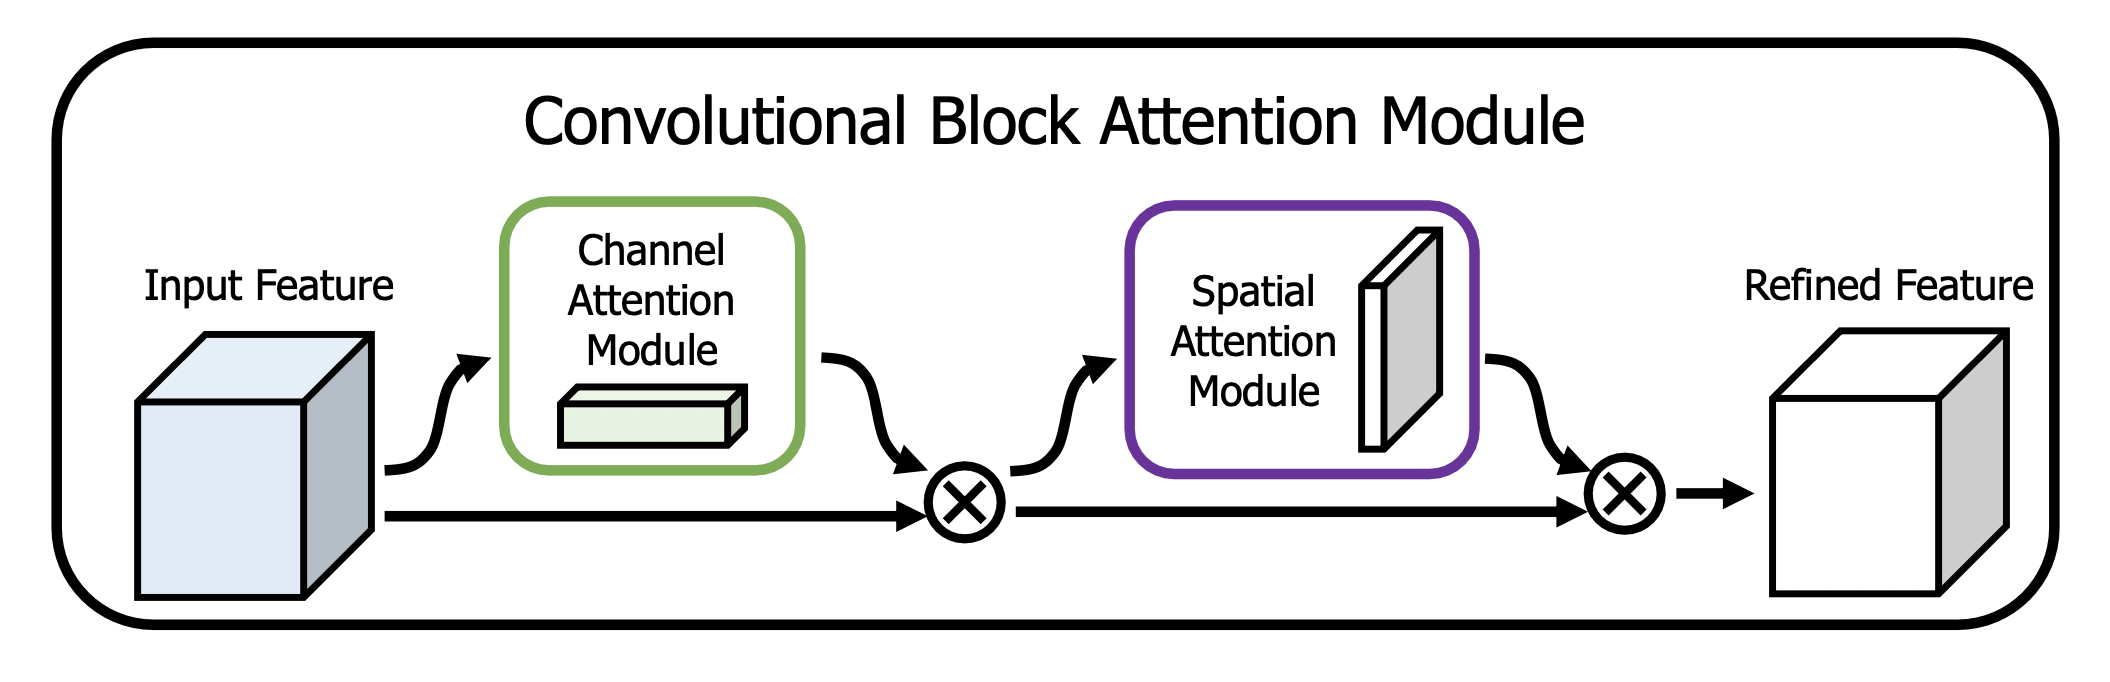
\includegraphics[width=\linewidth]{img/cbam}
	\caption{The overview of CBAM \cite{CBAM}}
	\label{fig:cbam}
\end{figure}

Given an intermediate feature map $ \textbf{F} \in \mathbb{R}^{C\times H \times W} $ as input, CBAM sequentially infers a 1D channel attention map $ \textbf{M}_c \in \mathbb{R}^{C\times 1 \times 1} $ and a 2D spatial attention map $ \textbf{M}_s \in \mathbb{R}^{1\times H \times W} $ as illustrated in Figure \ref{fig:cbam}. The overall attention process can be summarized as 
\begin{equation}
	\begin{split}
		\textbf{F}^\prime &= \textbf{M}_c (\textbf{F}) \otimes \textbf{F}\\
		\textbf{F}^{\prime \prime} &= \textbf{M}_s(\textbf{F}^\prime)\otimes \textbf{F}^\prime
	\end{split}
\end{equation} 
where $ \otimes $ denotes element-wise multiplication.



\subsection{Channel attention module}
\begin{figure}[h!]
	\centering
	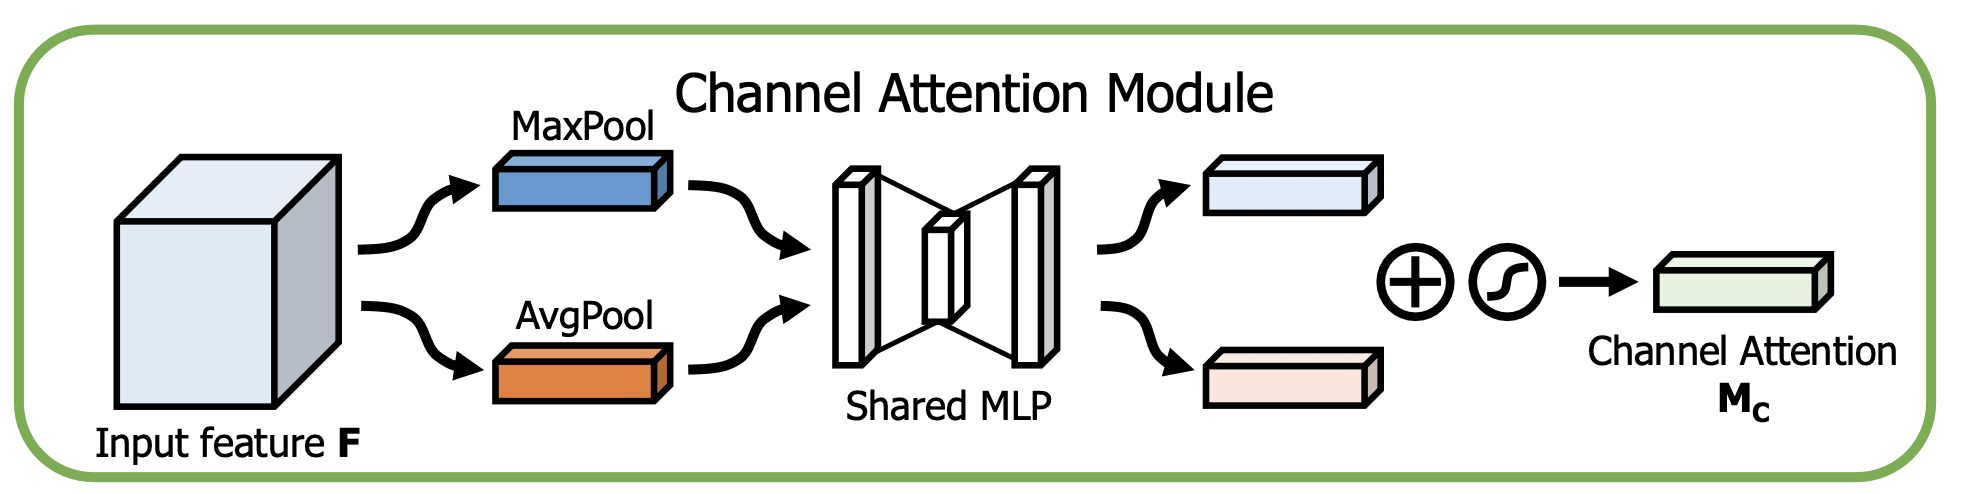
\includegraphics[width=\linewidth]{img/channel-attention-module}
	\caption{Diagram of channel attention module.\cite{CBAM}}
	\label{fig:channel-attention}
\end{figure}
The channel attention module focus on \textbf{what} is meaningful given an input image. To compute it, we first squeeze the \textcolor{BrickRed}{spatial dimension} of the input feature map. \cite{CAM} suggest to use average-pooling to learn the extent of the target object. \cite{CBAM} argues that max-pooling can be used to gather distinctive object features. Thus paper \cite{CBAM} exploits both average-pooling and max-pooling operations to aggregate spatial information.
$ \textbf{F}^c_{avg} $ denotes average-pooled features and $ \textbf{F}^c_{max} $ denotes max-pooled features. They are forwarded to a \textcolor{BrickRed}{shared network} (multi-layer perceptron (MLP)) to produce channel attention map $ \textbf{M}_c \in \mathbb{R}^{C\times 1\times 1} $. MLP has one hidden layer with hidden activation size $ \mathbb{R}^{C/r\times1\times1} $, where $ r $ is the reduction ratio.
Formally, the channel attention is computed as 
\begin{equation}
	\begin{split}
		\textbf{M}_c(\textbf{F}) &= \sigma(MLP(AvgPool(\textbf{F})) + MLP(MaxPool(\textbf{F})))\\
		&= \sigma(\textbf{W}_1(\textbf{W}_0(\textbf{F}_{avg}^c))+\textbf{W}_1(\textbf{W}_0(\textbf{F}^c_{max})))
	\end{split}
\end{equation} 


\subsection{Spatial attention module}
\begin{figure}[h!]
	\centering
	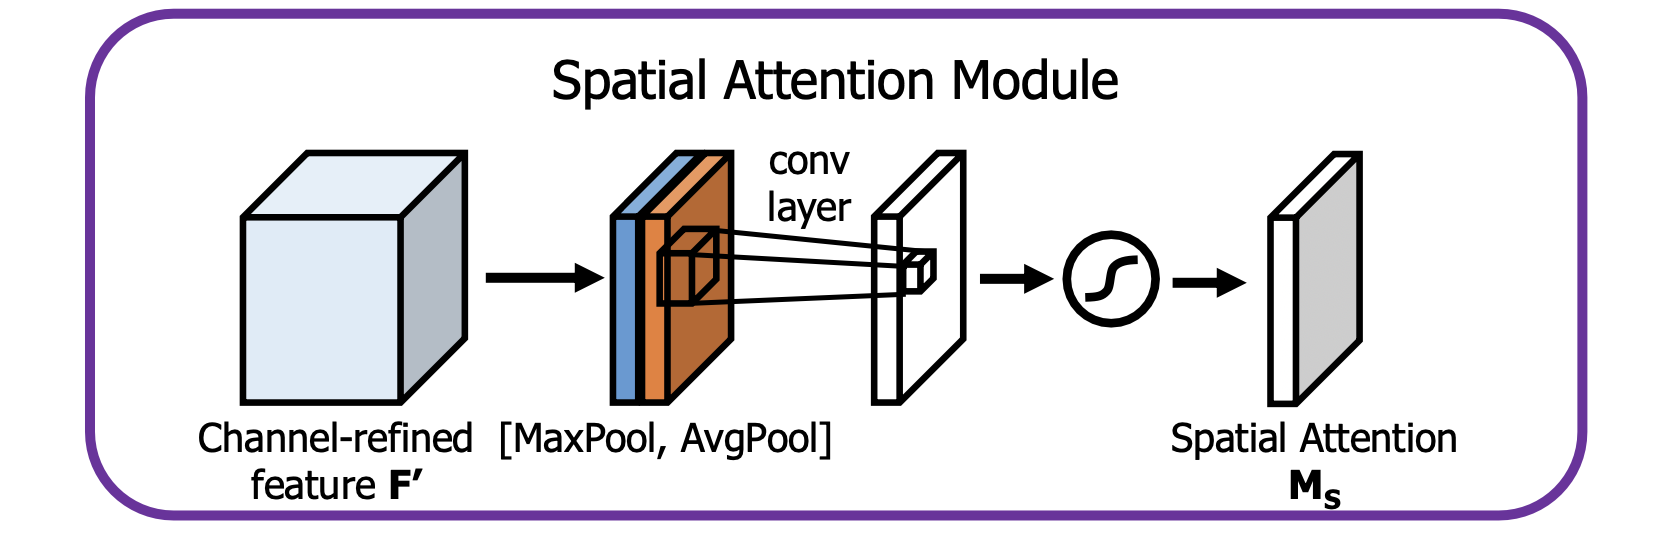
\includegraphics[width=\linewidth]{img/spatial-attention-module}
	\caption{Diagram of spatial attention module.\cite{CBAM}}
	\label{fig:spatial-attention}
\end{figure}
The spatial attention focuses on \textbf{where} is an informative part. \cite{attention-transfer} shows that applying pooling operations along the channel axis is effective in highlighting informative regions.
The spatial attention is computed as
\begin{equation}
	\begin{split}
		\textbf{M}_s(\textbf{F}) &= \sigma(f^{7\times7} ([AvgPool(\textbf{F}); MaxPool(\textbf{F})]))\\
		&= \sigma(f^{7\times 7}([\textbf{F}^s_{avg}; \textbf{F}^s_{max}]))
	\end{split}
\end{equation}
where $ \sigma $ denotes the sigmoid function and $ f^{7\times 7} $ represents a convolution operation with the filter size $ 7\times 7. $


\begin{figure}[h!]
	\centering
	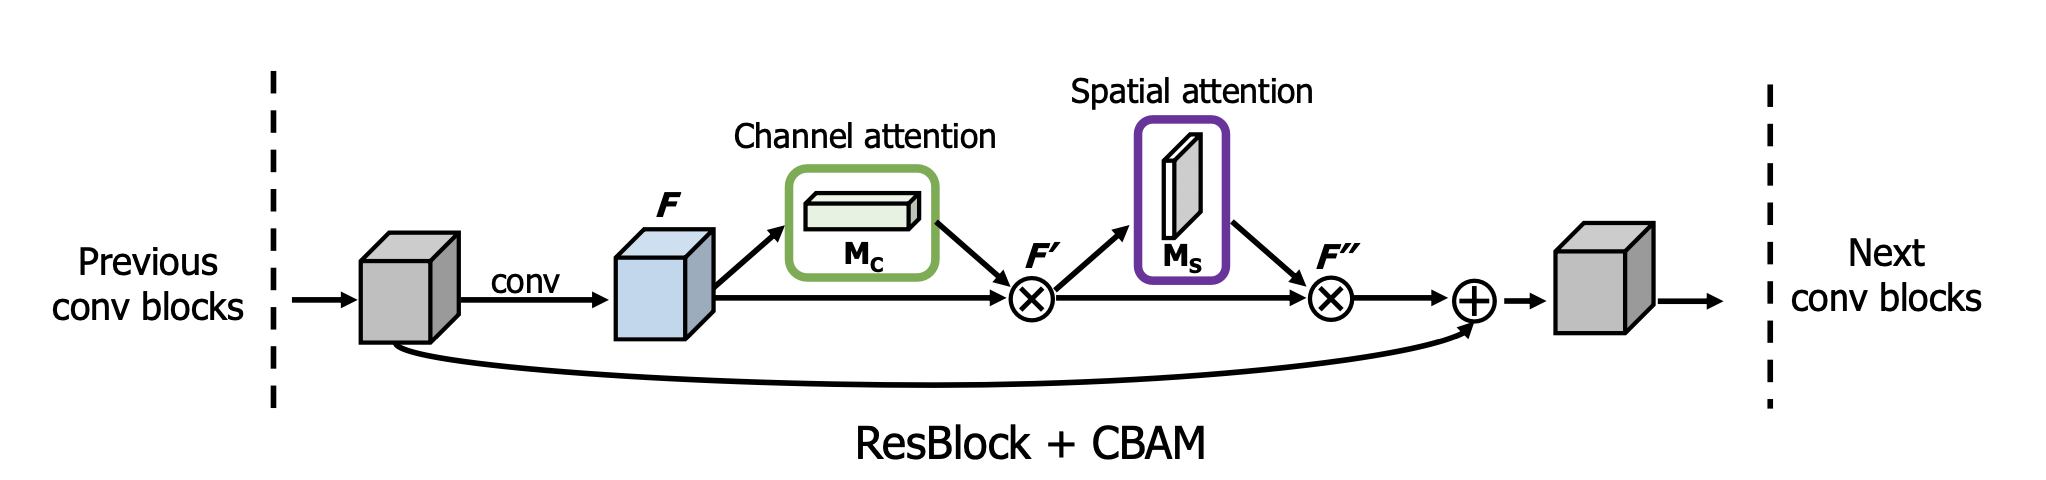
\includegraphics[width=\linewidth]{img/cbam-with-resblock}
	\caption{CBAM integrated with a ResBlock in ResNet.\cite{CBAM}}
	\label{fig:cbam-with-resblock}
\end{figure}



\section{Binarized Neural Network}

Let $ x^b $ be the binarized variable and $ x $ be the real-valued variable.. Deterministic binarization function
\begin{equation}
	\begin{split}
		x^b = Sign(x) = 
		\begin{cases}
				+1 & if\ x\ge 0 \\
				-1 & otherwise
		\end{cases}
	\end{split}
\end{equation}
Stochastic binarization function
\begin{equation}
	\begin{split}
		x^b = \begin{cases}
			+1 & \mbox{with probability}\ p =\sigma(x)\\
			-1 & \mbox{with probability}\ 1-p
		\end{cases}
	\end{split}
\end{equation}
where $ \sigma  $ is the \textit{hard sigmoid} function
\[\sigma(x) = \mbox{clip}(\frac{x+1}{2},0,1) = \max (0, \min(1,\frac{x+1}{2}))\]


\cite{BNN}





